\renewcommand*{\arraystretch}{1.1}

\subsection*{BI / read / 9}
\label{section:bi-read-09}

\noindent\begin{tabularx}{\queryCardWidth}{|>{\queryPropertyCell}p{\queryPropertyCellWidth}|X|}
	\hline
	query & BI / read / 9 \\ \hline
%
	title & Forum with related Tags
 \\ \hline
%
	pattern & \hfill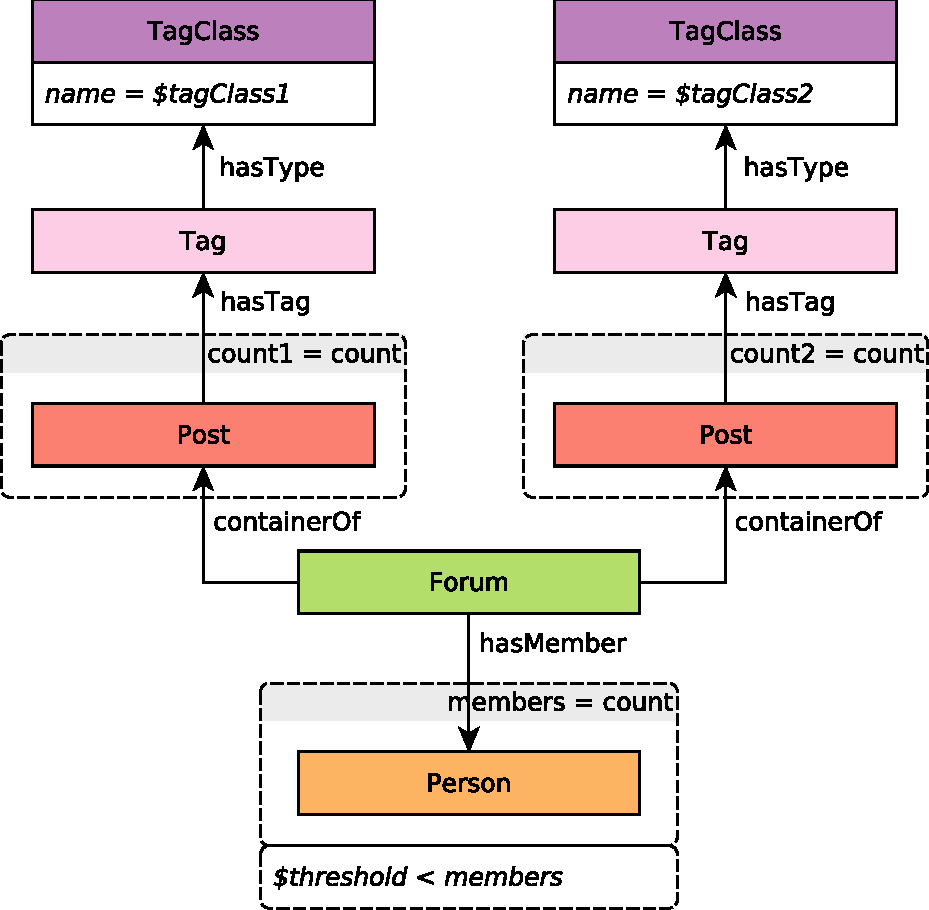
\includegraphics[scale=\patternscale,margin=0cm .2cm]{patterns/bi-read-09}\hfill\vadjust{} \\ \hline
%
	desc. & Given two \emph{TagClasses} (\texttt{tagClass1} and \texttt{tagClass2}),
find \emph{Forums} that contain at least one \emph{Post} with a
\emph{Tag} from \texttt{tagClass1} and at least one \emph{Post} with a
\emph{Tag} from \texttt{tagClass2} (direct children not transitive) --
this may be the same \emph{Post}.

Consider the \emph{Forums} with a number of members greater than a given
\texttt{threshold}. For every such \emph{Forum}, count the number of
\emph{Posts} that have a \emph{Tag} from \emph{TagClass1}
(\texttt{count1}), and the number of \emph{Posts} that have a \emph{Tag}
from \emph{TagClass2} (\texttt{count2}).
 \\ \hline
%
	
		params &
		\innerCardVSpace{\begin{tabularx}{\attributeCardWidth}{|>{\paramNumberCell}c|>{\varNameCell}M|>{\typeCell}m{\typeWidth}|Y|} \hline
		$\mathsf{1}$ & tagClass1
 & 32-bit Integer
 &  \\ \hline
		$\mathsf{2}$ & tagClass2
 & 32-bit Integer
 &  \\ \hline
		$\mathsf{3}$ & threshold
 & 32-bit Integer
 &  \\ \hline
		\end{tabularx}}\innerCardVSpace \\ \hline
	
%
	
		result &
		\innerCardVSpace{\begin{tabularx}{\attributeCardWidth}{|>{\resultNumberCell}c|>{\varNameCell}M|>{\typeCell}m{\typeWidth}|>{\resultOriginCell}c|Y|} \hline
		$\mathsf{1}$ & forum.id
 & 64-bit Integer
 & R &
				 \\ \hline
		$\mathsf{2}$ & count1
 & 32-bit Integer
 & R &
				Number of Posts with at least one tag belonging to tagClass1
 \\ \hline
		$\mathsf{3}$ & count2
 & 32-bit Integer
 & R &
				Number of Posts with at least one tag belonging to tagClass2
 \\ \hline
		\end{tabularx}}\innerCardVSpace \\ \hline
	
%
	
		sort		&
		\innerCardVSpace{\begin{tabular}{|>{\sortNumberCell}c|>{\varNameCell}l|>{\directionCell}c|} \hline
		$\mathsf{1}$ & abs(count2 - count1)
 & $\desc
$ \\ \hline
		$\mathsf{2}$ & forum.id
 & $\asc
$ \\ \hline
		\end{tabular}}\innerCardVSpace \\ \hline
	%
	limit & 100 \\ \hline
	%
	CPs &
	\multicolumn{1}{>{\raggedright}l|}{
		\chokePoint{1.2}, 
		\chokePoint{1.4}, 
		\chokePoint{2.1}, 
		\chokePoint{2.3}, 
		\chokePoint{2.4}
		} \\ \hline
	%
	%
\end{tabularx}
\queryCardVSpace